\chapter{Literature Review}\label{lit}
Numerous sports, like basketball \cite{skinner2010price} and baseball \cite{albert2010baseball}, have made use of artificial intelligence to glean insights from data and adjust their tactics. On the other hand, because it is a closed sector, football has only lately witnessed the integration of such technologies within its systems.
Data was previously ignored in this sport since the hierarchies are driven by professionals like former players and scouts. \cite{kuper2018soccernomics}

A plethora of studies attempted to forecast football match results by taking into account characteristics of the tournaments or leagues these matches were organized in. Although initially promising, as shown in some of the publications mentioned below, this strategy does not aid football teams in formulating plans during live matches.
Here are some examples of publications that explore this topic: 
\begin{itemize}
    \item Authors \citeauthor{5596458} \cite{5596458} stated that their study used an Artificial Neural Network to the dataset from the 2006 FIFA World Cup and claimed that if the drawn matches are not taken into account, an accuracy of 76.9\% may be attained. This investigation established a standard for football statistics. It is essential to remember that every football tournament is unique, and training a model for every competition is not creative. 
    \item Authors \citeauthor{joseph2006predicting} \cite{joseph2006predicting} study aims to predict game outcomes for the Tottenham Hotspur football team. In addition to Decision Tree algorithm and the K-nearest neighbours method, a Bayesian network was used in the implementation. The Bayesian Network fared better than other algorithms in terms of prediction accuracy in this domain, according to the authors' research. The study's overall accuracy came at 59.21\%. (win, draw or lose). 
    \item  Genetic programming was used by \citeauthor{6604116} \cite{6604116} to predict the outcomes of English Premier League games, which may end in a win, loss, or a tie. As an input to the Genetic Program system, they selected 25 traits from each game, and the system then created a function to predict the result. A single GP-generated function's prediction accuracy underwent an experimental test, and the results looked good. For each League game played for each season, this study manually fed 25 different characteristics. The shortcomings of forecasting football games are shown by this as well as the fact that the resultant accuracy was 70\%. 
    \item To find non-linear correlations, authors \citeauthor{rotshtein2005football} \cite{rotshtein2005football} created a model that uses fuzzy logic as the foundation. To fine-tune fuzzy rules and get acceptable simulation results, they used competition data. The tuning method involved determining the parameters of the fuzzy membership functions and rule weights using a combination of genetic and neural optimization approaches. The model is promising, but it does not take into account variables like injured players, players who have been booked and benched, referee prejudice, and weather conditions. Additionally, owing to its nature, it only forecasts results based on previous matches. 
\end{itemize}

These publications made it simple to understand how football match prediction models take into account variables that have nothing to do with the tactics used, but rather with the patterns and results of earlier games. This went against the objective of the case study. 

\begin{figure}[!h]
    \centering
    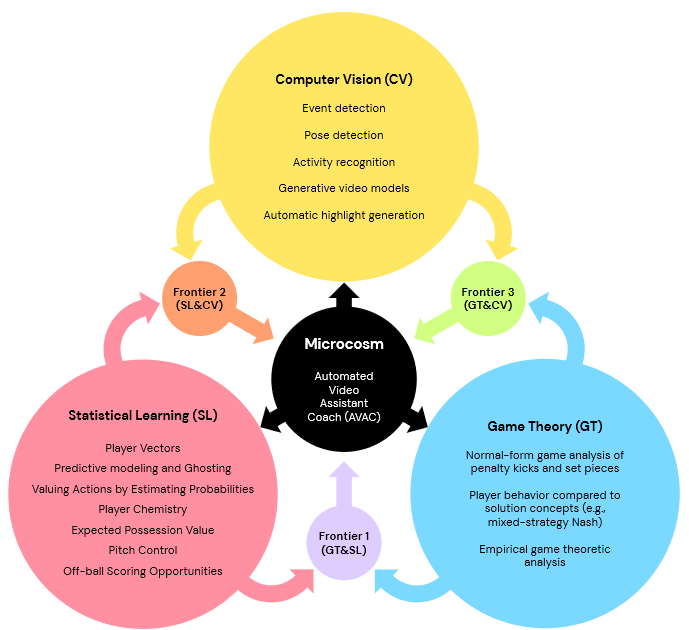
\includegraphics[scale=0.75]{images/deepmind.PNG}
    \caption{Proposed model by deepmind}
    \label{fig:my_label}
    \cite{DBLP:journals/corr/abs-2011-09192}
\end{figure}

The study carried out by DeepMind Technologies, a division of Alphabet Inc. \cite{DBLP:journals/corr/abs-2011-09192}, illustrates the present impact of several branches of artificial intelligence on football analytics. As shown in the graphic  \ref{fig:my_label}, statistical learning, computer vision, and game theory work together to produce a possible system for football analytics that has the potential to spark a data revolution.

This case study sought to demonstrate statistical learning using the Expected Goal (xG) measure, which Vic Barnett and Sarah Hilditch initially introduced in their 1993 publication. \cite{barnett1993effect}

\begin{figure}[!h]
    \centering
    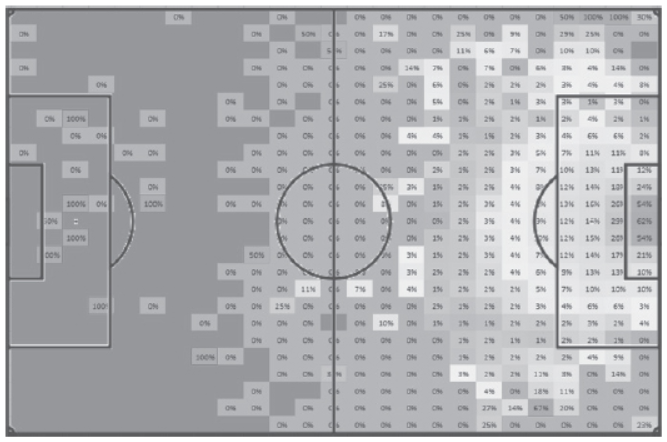
\includegraphics[scale=.75]{images/shot analysis.PNG}
    \caption{Shot Analysis}
    \label{fig:shot analysis}
    \cite{biermann2019football}
\end{figure}

In his work, the author \citeauthor{biermann2019football} has offered a thorough explanation of how football strategies are developed using the xG measure. Football is a game of probability, as was stated in the previous section \ref{football}. The likelihood that a wonder goal will be scored from various locations on the football field is shown in the figure \ref{fig:shot analysis}. The application of xG metric is demonstrated in this investigation. The shot's viewpoint was also taken into account in order to give this statistic additional context. For instance, shots from a distance of 12 yards have a higher likelihood of being successful than headers do, as do shots from counterattacks since the opposing defence is more unfocused in these circumstances. There are specific probability for attempts made in dead-ball situations as well. 

Additionally, as seen in figure \ref{fig:expectedgoals}, the work \cite{biermann2019football} has also emphasised time series graphs that indicate how goals scored correspond to goal scoring possibilities. 

\begin{figure}[!h]
    \centering
    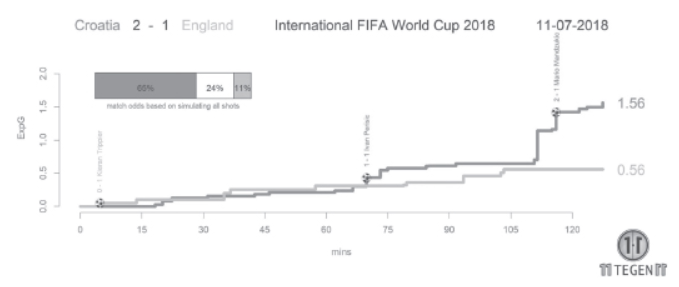
\includegraphics[scale=0.75]{images/expected goals.png}
    \caption{Time Series Graph}
    \label{fig:expectedgoals}
    \cite{biermann2019football}
\end{figure}

These methods have aided managers and coaches in putting tactics into practise that have improved player placement and game play. 

\citeauthor{rathke2017examination} looked at goals scored in European football leagues to determine whether factors are related to predicting expected goals (xG). This idea helped them evaluate players, especially strikers, according to the number of goals they score year after year. As a consequence, this research examined shots from 380 and 306 Premier League and Bundesliga games played in the 2012–2013 seasons, respectively. On the playing field, all of the shots were separated into regions, and each region was given a hypothetical goal value. The shot's distance from the goal and angle with respect to the goal were two factors that were looked at. It was postulated that the shots' range and aiming angle had an impact on the calculation of xG. \cite{rathke2017examination} The middle-of-the-table teams' goals and goals against were precisely identified by the algorithm. Teams at the top and bottom performed poorly, correspondingly. 

The model created in \cite{rathke2017examination} only took into account two aspects, but it may still be improved. Additionally, it hasn't been tested with newer data. 

\begin{figure}[!h]
    \centering
    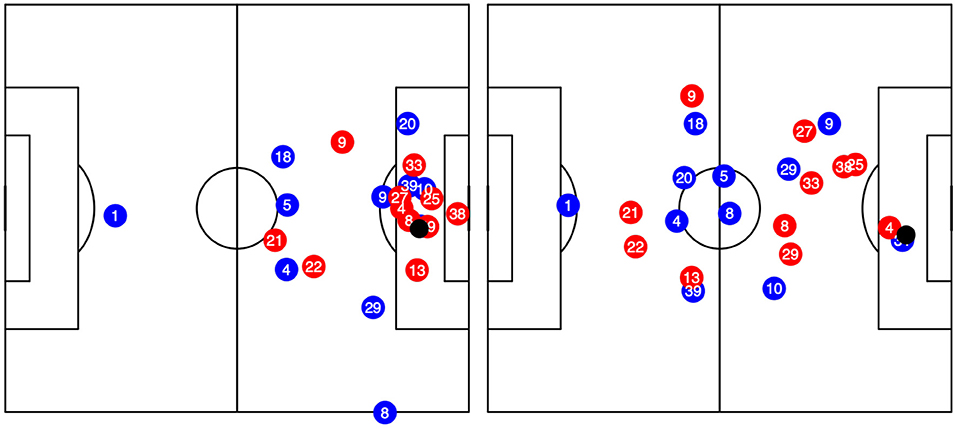
\includegraphics[scale=0.35]{images/anzer.jpg}
    \caption{Gabriel Anzer and Pascal Bauer}
    \label{Gabriel Anzer}
    \cite{anzer2021goal}
\end{figure}

The authors \citeauthor{anzer2021goal} assessed the calibre of each individual shot in their own model that investigates the xG metric. \cite{anzer2021goal} Their strategy has been examined by seasoned football experts and scientifically proven. The best model uses the XGBoost methodology and was constructed using precisely calibrated parameters obtained from synchronizing positional and event data of 105,627 shots in the Football League played in Germany. More precision than any other model that has been formally published may be shown in this model. This model has a 0.197 RPS (ranked probability score). 

Another study \cite{madrero2020creating} considered the ability of the shooter from different data-sets. The features that this considered were, Long Shots, Finishing, Heading, Shooting and Weak Foot. Along with these features there were other features that includes, x and position of the player, player ability, post rebound, back pass etc. An ANN (Artificial Neural Network) was implemented along with XGBoost algorithm and Logistic Regression with XGBoost performing the best. Due to lack of data the models were rather poor in performance. The best performing model for this study was XGBoost Algorithm.

\begin{figure}[!h]
    \centering
    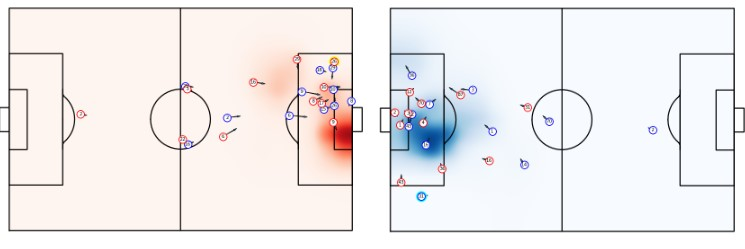
\includegraphics[scale=0.75]{images/spear.jpg}
    \caption{Time Series Graph}
    \label{Off Ball Scoring}
    \cite{spearman2018beyond}
\end{figure}


Many methods have been developed to assess the quality of soccer shots. In this work, we assess the efficiency of off-ball positioning prior to shoots that potentially result in goals. Consider a tall, unmarked centre forward who is positioned near the far post during a corner kick. When the cross comes in, the centre forward simply heads it in; other times, the cross sails over his head. Another example is a winger playing onside while breaking through the defensive line. Sometimes the through-ball arrives; other times, the winger may cut their run short when a teammate fails to provide a timely pass. Even though they never got the ball, the offensive player has generated a chance in both cases. The author \citeauthor{spearman2018beyond} \cite{spearman2018beyond} built a probability and physics-based model that leverages spatiotemporal player monitoring data to assess such off-ball scoring possibilities in this research (OBSO). This model may be used to predict which players, if any, are most expected to score at any moment throughout the game, as well as where on the field they are likely to score. The author demonstrates three significant applications of their model:
\begin{enumerate}
    \item Identifying and analysing key opportunities throughout a game
    \item to aid opposition analysis by indicating areas of the pitch where individual players or clubs are more likely to produce off-ball scoring chances.
    \item to automate talent discovery by identifying players throughout a whole league who excel at providing off-ball scoring opportunities. 
\end{enumerate}

\section{Summary}
The studies analysed in this section consolidated the nature of this case study and confirmed that the direction undertaken is a fruitful path with a lot of potential answers to how data science can be used in football. Furthermore, the works analysed in this study also highlight the future work of the metric that was developed in this study.